%----------------------------------------------------%
%              DISEÑO E IMPLEMENTACIÓN               %
%----------------------------------------------------%

\chapter{Diseño e Implementación}
\label{diseno-e-implementacion}

Añadir descripcion del apartado.\\

\section{Estructura del proyecto}
\label{diseno-e-implementacion:estructura}

En este apartado se revisara la estructura del proyecto, es decir, los ficheros que componen el proyecto y su estructura de carpetas. En la figura ~\ref{fig:files-1} se muestra la raíz del proyecto:\\

\begin{figure}[h]
	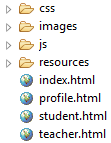
\includegraphics{files-1}
	\caption{Raíz del proyecto}
	\label{fig:files-1}
\end{figure}

El proyecto cuenta con 4 carpetas principales: css, js, images y resources. Además contiene 4 ficheros HTML:

\begin{itemize}
\item \textbf{index.html:} funciona como pantalla de identificación de usuario y permite redirigir a las vistas principales (teacher.html o student.html) dependiendo del rol del usuario identificado.
\item \textbf{student.html:} es la vista del alumno.
\item \textbf{teacher.html:} es la vista del profesor.
\item \textbf{profile.html:} pantalla de perfil del profesor, únicamente accesible desde teacher.html.
\end{itemize}

Dentro de las otras carpetas encontramos más ficheros.

\begin{figure}[h]
\begin{subfigure}[b]{0.5\textwidth}
	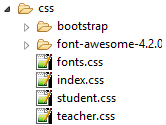
\includegraphics[width=0.4\linewidth]{files-css}
	\caption{Contenido de la carpeta css}
	\label{fig:files-css}
\end{subfigure}
%
\begin{subfigure}[b]{0.5\textwidth}
	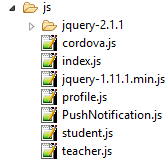
\includegraphics[width=0.4\linewidth]{files-js}
	\caption{Contenido de la carpeta js}
	\label{fig:files-js}
\end{subfigure}
%
\begin{subfigure}[b]{0.5\textwidth}
	
\includegraphics[width=0.4\linewidth]{files-images}
	\caption{Contenido de la carpeta images}
	\label{fig:files-images}
\end{subfigure}
%
\begin{subfigure}[b]{0.5\textwidth}
	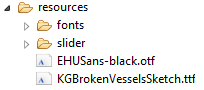
\includegraphics[width=0.4\linewidth]{files-resources}
	\caption{Contenido de la carpeta resources}
	\label{fig:files-resources}
\end{subfigure}

\caption{Contenido de la carpetas principales de la raíz del proyecto}
\label{fig:files-2}
\end{figure}

\section{Interfaces o lado del cliente}
\label{diseno-e-implementacion:interfaces}

Hablar sobre la parte del cliente, las interfaces y el javascript.\\

\section{Lógica de negocio o lado del servidor}
\label{diseno-e-implementacion:logica-negocio}

Hablar sobre la parte de servidor y la base de datos.\\

\subsection{Base de datos}
\label{diseno-e-implementacion:logica-negocio:bd}

El diseño de la base de datos se ha realizado considerando desarrollos anteriores del grupo GaLan.
Por ello muchos de los elementos son comunes con una de sus herramientas genérica de creación
de sistemas docente, MAGADI, que ha sido proporcionada para este proyecto.\\

Se han incorporado unas tablas nuevas a la base de datos ya existente para la gestión de ejercicios.\\